\subsection{Infrastrukturen}

\subsubsection{Recherchegrund}

Mit der Recherche über bestehende Infrastrukturen in Hochhäusern können wir beurteilen, wie unsere Turbine am besten darin integriert wird.



\subsubsection{Ergebnisse}
\paragraph{Fachbegriffe}
\begin{table}[H]

\begin{tabular}{|l|l|lll}

\cline{1-2}

Fallleitung   & \begin{tabular}[c]{@{}l@{}}Eine senkrecht nach unten führende Abwasserleitung führt meist in\\   Grundleitung oder Sammelleitung\end{tabular}                                                                                                      &  &  &  \\ \cline{1-2}

Verziehung    & Seitliche Versetzung einer Fallleitung                                                                                                                                                                                                              &  &  &  \\ \cline{1-2}

Sammelleitung & \begin{tabular}[c]{@{}l@{}}Horizontale Abwasserleitung, die innerhalb eines Gebäudes mehrere\\   Abwasserquellen zusammenführt\end{tabular}                                                                                                         &  &  &  \\ \cline{1-2}

Grundleitung  & \begin{tabular}[c]{@{}l@{}}Horizontale Abwasserleitung, die unter dem Gebäude oder auf dem\\   Grundstück im Boden verlegt ist; Unterste Leitung auf Privatgrundstück. \\ \cite{shk-journal} \end{tabular} &  &  &  \\ \cline{1-2}

Hochhaus      & \begin{tabular}[c]{@{}l@{}}Schweiz: Gebäude mit einer Gesamthöhe von über 30 Metern.\\   Deutschland: Gebäude mit\\   einem Aufenthaltsraum, dessen Fussboden mindestens 22 Meter über dem Erdboden\\   liegt.\end{tabular}                         &  &  &  \\ \cline{1-2}

Nennweite     & Innendurchmesser eines Rohrs                                                                                                                                                                                                                        &  &  &  \\ \cline{1-2}

\end{tabular}

\end{table}

\paragraph{Fallleitungen, Beruhigungsstrecken und Verziehungen}
Durch Luftwiderstand und Reibung im Rohr beträgt die maximale Fallgeschwindigkeit, die in einer Fallleitung bei 15 Meter Fallhöhe erreicht wird, etwa 10 m/s. Deshalb muss in Hochhäusern das Abwasser nur am Ende einer Fallleitung abgebremst werden, unmittelbar bevor es einer Sammel- oder Grundleitung zugeführt wird. Die Abbremsung erfolgt durch eine sogenannte Beruhigungsstrecke, zwei 45° Winkel mit einem Zwischenstück von 250 mm am Ende der Fallleitung. (Siehe Abbildung \ref{fig:Falleitungen}) Unsere Turbine sollte deshalb vor oder anstelle dieser Beruhigungsstrecke eingebaut werden.
\cite{baunetzwissen}

\begin{figure}[H]
	\centering
	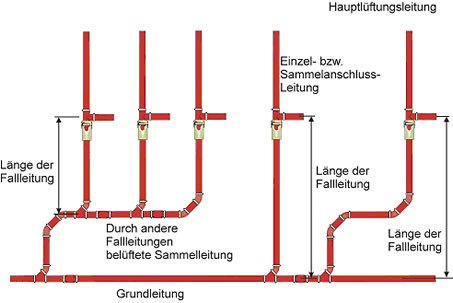
\includegraphics[width=10cm]{Falleitungen_1.jpg}
	\caption{Schematische Verlegung von Fallleitungen \cite{baunetzwissen}}
	\label{fig:Falleitungen}
	
\end{figure}

Da durch die baulichen Gegebenheiten nicht immer ein senkrechter Verlauf der Fallleitung möglich ist, sind Verziehungen erforderlich. Eine Verziehung ist eine horizontale Versetzung der Fallleitung. \cite{docplayer}

Bei einer Verziehung kommt es auch zur Abbremsung des fallenden Abwassers. Deshalb sollte in den Letzten 15 Metern über der Turbine keine Verziehung mehr vorhanden sein, damit das Abwasser seine maximale Fallgeschwindigkeit erreichen kann.

\paragraph{Entlüftung}
In Fallleitungen werden grosse Luftvolumen bewegt, bei einer Nennweite DN 100 und einer Abwasserbelastung von beispielsweise 100 L/min werden 2340 L/min Luft mitgeführt.\cite{docplayer}
Diese Luftmenge behindert den Fluss des Abwassers, weshalb die Rohrleitungen belüftet werden müssen, damit ein Luftaustausch stattfinden kann. Auch muss verhindert werden, dass in den Leitungen Über- oder Unterdruck entsteht, da sonst ein Siphon leer gesaugt werden könnte. Dazu gibt es mehrere Lösungen, wobei nicht alle dazu geeignet sind, unsere Turbine einzubauen. Ein Geberit Sovent Formstück (siehe Abbildung \ref{fig:Sovent}) braucht wenig Platz, keine zusätzlichen Entlüftungsrohre und erlaubt mehr Durchfluss, da der Druckausgleich innerhalb Fallleitung geschieht. Es wird in jedem Stockwerk in die Fallleitung eingebaut und führt die Sammelleitungen des Stockwerkes in die Falleitung ein. Dies hat aber für uns aber den Nachteil, dass das Abwasser in jedem Stockwerk abgebremst wird und so nie seine Maximalgeschwindigkeit erreicht.

\begin{figure}[H]
    \centering
    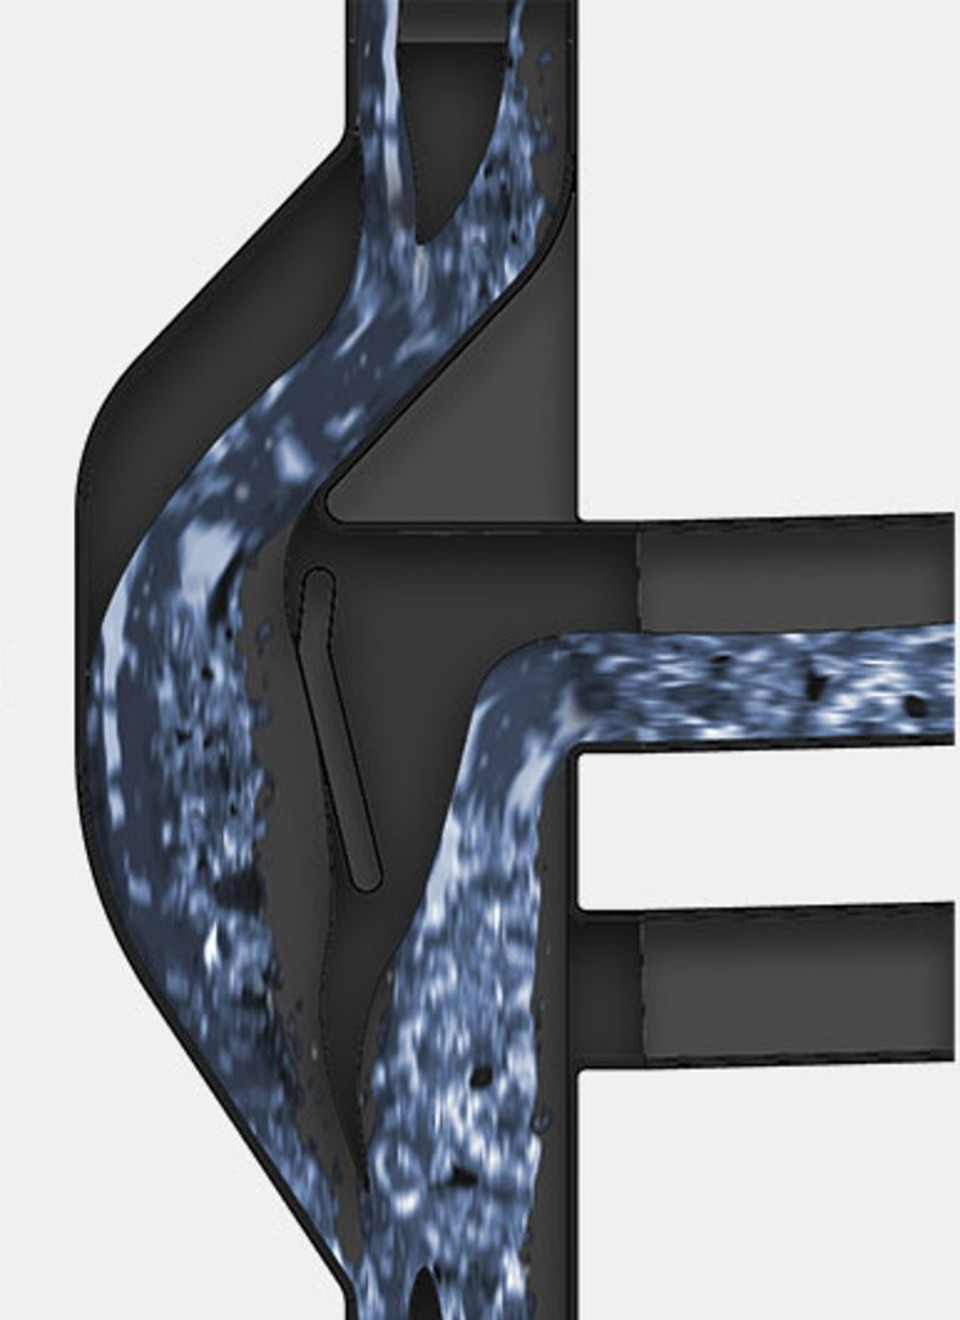
\includegraphics[width=6cm]{Geberit_PE_Sovent_Formstueck.jpg}
    \caption{Geberit Sovent Formstück \cite{geberit}}
	\label{fig:Sovent}
\end{figure}

Die anderen üblichen Entlüftungsarten sollten für uns kein Problem darstellen, da das Wasser im Fall nicht gebremst wird. (Siehe Abbildung \ref{fig:Entlüftungsarten})

\begin{figure}[H]
\centering
\subfloat[Direkte Nebenlüftung]{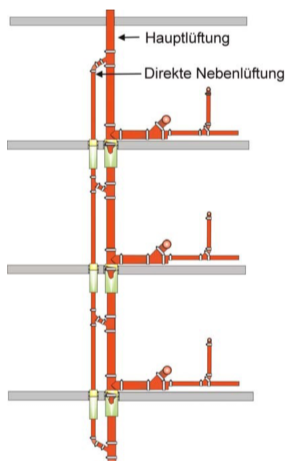
\includegraphics[width=5cm]{Direkte_Nebenlueftung.PNG}}\;
\subfloat[Indirekte Nebenlüftung]{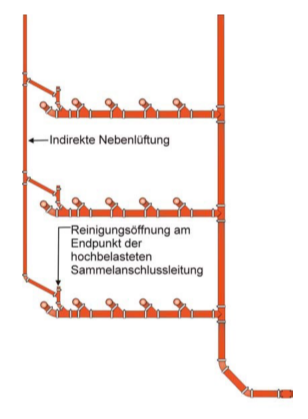
\includegraphics[width=5cm]{Indirekte_Nebenlueftung.PNG}}\;
\subfloat[Sekundärlüftung]{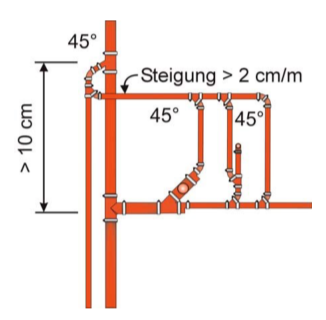
\includegraphics[width=4cm]{Sekundaerlueftung.PNG}}
\caption{Verschiedene Entlüftungsarten \cite{docplayer}}
\label{fig:Entlüftungsarten}
\end{figure}

\paragraph{Abwassermengen}
Der Durchschnittsverbrauch an Trinkwasser beträgt für Wohnungen mit Bad 150 L/pro Person und Tag. \cite{wohnbau} Der grösste Teil dieser Wassermenge wird als Abwasser wieder entsorgt. 
\newline
Aufteilung:
\newline
- 48 L \; WC-Spülung
\newline
- 43 L \; Baden und Duschen
\newline
- 25 L \; Wäschewaschen und Geschirrspülen
\newline
- 03 L \;  Trinken und Kochen
\newline


Ein Hochhaus mit beispielsweise 200 Bewohnern produziert also etwa 30 Kubikmeter Abwasser am Tag.

\subsubsection{Fazit}
Um die Fallgeschwindigkeit des Wassers optimal auszunutzen, sollte die Turbine am Ende einer Fallleitung eingebaut werden. Oberhalb der Turbine muss das Wasser mindestens 15 Meter hoch frei fallen können, ohne durch Verziehungen abgebremst zu werden, damit es seine Maximalgeschwindigkeit erreichen kann. 


\clearpage 






